% =====================================================================
%  Praktikumsbericht – Neffy 3.0 (Team Sensorik)
%  Bachelor Humanoide Robotik (HROB), BHT Berlin
%
%  Kompilieren: in VS Code mit LaTeX Workshop speichern (Strg+S) oder
%  Strg+Alt+B; PDF-Vorschau: Strg+Alt+V.
%  Ablauf: pdflatex -> biber -> pdflatex -> pdflatex
% =====================================================================
\documentclass[
  a4paper,
  12pt,
  oneside,
  parskip=half,
  toc=listof,        % Verzeichnisse im Inhaltsverzeichnis
  toc=bibliography,
  listof=totoc,
  numbers=noenddot,  % „2.1 Titel“ statt „2.1. Titel“ (wie Vorlage)
]{scrreprt}

% --- Sprache und Schrift ---------------------------------------------
\usepackage[T1]{fontenc}
\usepackage[utf8]{inputenc}
\usepackage[ngerman]{babel}
\usepackage{lmodern}
\usepackage{microtype}
\usepackage[autostyle]{csquotes}

% --- Seitenlayout ----------------------------------------------------
\usepackage[
  left=3cm, right=3cm, top=2.5cm, bottom=2.5cm,
  marginparwidth=2.4cm,
]{geometry}

% Kopfzeile wie im Praxisbericht Neffy 2:
% links Kapitel, rechts Berichtstitel, Seitenzahl unten mittig
\usepackage[headsepline]{scrlayer-scrpage}
\pagestyle{scrheadings}
\automark{chapter}
\clearpairofpagestyles
\ihead{\leftmark}
\ohead{Praktikumsbericht Neffy 3.0}
\cfoot*{\pagemark}
\renewcommand*{\chapterpagestyle}{scrheadings}
\setkomafont{pageheadfoot}{\normalfont\small}
% Überschriften in Serifenschrift (wie Vorlage)
\setkomafont{disposition}{\normalfont\bfseries}

% --- Abbildungen, Tabellen, Diagramme --------------------------------
\usepackage{graphicx}
\graphicspath{{abbildungen/}}
\usepackage{caption}
\usepackage{subcaption}
\usepackage{booktabs}
\usepackage{array}
\usepackage{float}
\usepackage{xcolor}
\usepackage{tikz}
\usetikzlibrary{positioning, arrows.meta}
\usepackage{pgfplots}
\pgfplotsset{compat=1.18}
\usepackage{siunitx}
\usepackage{amssymb}    % \checkmark in der Evaluation
\sisetup{locale=DE}

% --- Code-Auszüge ----------------------------------------------------
\usepackage{listings}
\lstset{
  basicstyle=\ttfamily\footnotesize,
  numbers=left, numberstyle=\tiny, frame=single,
  breaklines=true, columns=fullflexible,
  literate={ä}{{\"a}}1 {ö}{{\"o}}1 {ü}{{\"u}}1 {ß}{{\ss}}1
           {Ä}{{\"A}}1 {Ö}{{\"O}}1 {Ü}{{\"U}}1,
}

% --- Offene Punkte ---------------------------------------------------
% Für die Abgabe: [disable] setzen, dann verschwinden alle Marker.
\usepackage[colorinlistoftodos, ngerman]{todonotes}
\setuptodonotes{size=\footnotesize}
\newcommand{\todoi}[1]{\todo[inline]{#1}}

% Platzhalter für noch fehlende Abbildungen
\newcommand{\platzhalter}[2][0.8\linewidth]{%
  \fbox{\parbox[c][4cm][c]{#1}{\centering\small\textit{Platzhalter:}\\ #2}}}

% --- Abkürzungen -----------------------------------------------------
\usepackage{acro}
\acsetup{
  make-links = true,
  list/display = all,
  list/heading = chapter*,
  list/name = Abkürzungsverzeichnis,
}
% ---------------------------------------------------------------------
%  Abkürzungen (Paket acro)
%  Im Text: \ac{FDM} -> beim ersten Mal ausgeschrieben, danach kurz.
% ---------------------------------------------------------------------
\DeclareAcronym{ADC}{short = ADC, long = Analog-Digital-Umsetzer}
\DeclareAcronym{BHT}{short = BHT, long = Berliner Hochschule für Technik}
\DeclareAcronym{CAD}{short = CAD, long = Computer-Aided Design}
\DeclareAcronym{CRC}{short = CRC, long = Cyclic Redundancy Check}
\DeclareAcronym{DSI}{short = DSI, long = Display Serial Interface}
\DeclareAcronym{FDM}{short = FDM, long = Fused Deposition Modeling}
\DeclareAcronym{FSR}{short = FSR, long = Force Sensing Resistor}
\DeclareAcronym{GPIO}{short = GPIO, long = General Purpose Input/Output}
\DeclareAcronym{KI}{short = KI, long = Künstliche Intelligenz}
\DeclareAcronym{MRI}{short = MRI, long = Mensch-Roboter-Interaktion}
\DeclareAcronym{I2C}{short = I\textsuperscript{2}C, long = Inter-Integrated Circuit}
\DeclareAcronym{LED}{short = LED, long = Leuchtdiode, long-plural-form = Leuchtdioden}
\DeclareAcronym{PIR}{short = PIR, long = Passiv-Infrarot}
\DeclareAcronym{PLA}{short = PLA, long = Polylactid}
\DeclareAcronym{PTAT}{short = PTAT, long = Proportional to Absolute Temperature}
\DeclareAcronym{STAI}{short = STAI, long = State-Trait Anxiety Inventory}
\DeclareAcronym{ToF}{short = ToF, long = Time of Flight}
\DeclareAcronym{UART}{short = UART, long = Universal Asynchronous Receiver Transmitter}


% --- Literatur -------------------------------------------------------
\usepackage[
  backend=biber,
  style=numeric,
  sorting=none,
  urldate=long,
]{biblatex}
\addbibresource{literatur.bib}

% --- Links (zuletzt laden) -------------------------------------------
\usepackage[hidelinks]{hyperref}

% =====================================================================
\begin{document}

\pagenumbering{Roman}
% ---------------------------------------------------------------------
%  Titelblatt nach Vorlage Praxisbericht Neffy 2 (BHT-Stil)
%  bht_titelseite.pdf = BHT-Logo, Formen und „Studiere Zukunft“ als
%  ganzseitiger Hintergrund (aus der Vorlage, Text entfernt).
%  Alle Zeilen sind fest positioniert (Abstand von oben, wie Vorlage).
% ---------------------------------------------------------------------

% Kompakter Marker für offene Felder (erscheint auch in der Todo-Liste)
\newcommand{\titelfehlt}[1]{%
  \colorbox{orange!50}{\strut #1}%
  \addcontentsline{tdo}{todo}{Titelblatt: #1}}

% Matrikelnummern stehen nur lokal in matrikelnummern.tex (per .gitignore
% ausgeschlossen, öffentliches Repo), z. B.:
%   \newcommand{\matrEddy}{123456}
%   \newcommand{\matrYounes}{654321}
\InputIfFileExists{matrikelnummern}{}{}
\providecommand{\matrEddy}{\titelfehlt{Matrikelnummer}}
\providecommand{\matrYounes}{\titelfehlt{Matrikelnummer}}

% \titelzeile{Abstand von oben}{Inhalt}
\newcommand{\titelzeile}[2]{%
  \node[anchor=base west, inner sep=0pt]
    at ([xshift=3.62cm, yshift=-#1]current page.north west) {#2};}

\begin{titlepage}
  \begin{tikzpicture}[remember picture, overlay]
    \node[anchor=north west, inner sep=0pt] at (current page.north west)
      {
\includegraphics[width=\paperwidth]{bht_titelseite}};

    \titelzeile{12.78cm}{\fontsize{23}{28}\selectfont Praktikumsbericht -- Neffy 3.0}
    \titelzeile{13.75cm}{\large Labor für Kommunikation}
    \titelzeile{14.55cm}{\large Team Sensorik}

    \titelzeile{16.40cm}{\large vorgelegt von:}

    \titelzeile{17.45cm}{\large\textbf{Eddy Werk}}
    \titelzeile{18.10cm}{\large Matr.-Nr.: \matrEddy}

    \titelzeile{19.17cm}{\large\textbf{Younes Jamil}}
    \titelzeile{19.82cm}{\large Matr.-Nr.: \matrYounes}

    \titelzeile{21.30cm}{\large
      \begin{tabular}[t]{@{}l l@{}}
        \textbf{Lehrkraft:}   & Prof.\ Dr.\ Ilona Buchem \\
        \textbf{Betreuer:}    & Prof.\ Dr.\ Manfred Hild \\
        \textbf{Studiengang:} & Bachelor Humanoide Robotik \\
      \end{tabular}}

    \titelzeile{25.17cm}{\large Abgabe am 27.~Oktober 2026}
  \end{tikzpicture}
  \null
\end{titlepage}


\tableofcontents

% Übersicht aller offenen Punkte – vor der Abgabe entfernen
\listoftodos[Offene Punkte (vor Abgabe entfernen)]

\clearpage
\pagenumbering{arabic}

% =====================================================================
%  Kapitel 1 – Einleitung (~1 Seite)
% =====================================================================
\chapter{Einleitung}
\label{kap:einleitung}

Stress betrifft sehr viele Menschen, sei es durch Arbeit, Studium oder belastende
Lebensumstände. Eine einfache Möglichkeit, Anspannung zu begegnen, sind angeleitete
Atemübungen mit einem ruhigen, gleichmäßigen Rhythmus aus Ein- und Ausatmen. Soziale Roboter
können solche Übungen nicht nur über Bild und Ton anleiten, sondern den Atemrhythmus auch
körperlich spürbar machen. Der an der Yale University entwickelte Roboter Ommie gibt Einatmen,
Halten und Ausatmen über haptische Interaktion und Audio vor~\cite{matheus2022ommie}. Im Labor
für Kommunikation der \ac{BHT} wurde dieses Prinzip mit Neffy aufgegriffen: In einer
Pilotstudie mit Neffy~1.0 sanken die Angstwerte der Teilnehmenden nach der Übung
signifikant~\cite{thomas2025neffy}. In einer Studie mit 14 Geflüchteten aus der Ukraine
empfanden die Teilnehmenden ihren Stress nach einer Übung mit Neffy~2.0 als deutlich geringer
als nach einer reinen Audioanleitung~\cite{buchem2026neffy2}.

Die Zielgruppe von Neffy ist bewusst weit gefasst. Denkbar ist der Einsatz im Alltag ebenso
wie bei Kindern oder bei besonders belasteten Gruppen wie in der Studie zu Neffy~2.0. Ein
Anliegen des Gesamtprojekts ist es, herauszufinden, in welchen Anwendungsfällen ein solcher
Roboter am meisten Sinn ergibt; möglich sind später auch verschiedene Varianten für
unterschiedliche Einsatzbereiche. Neffy~3.0 ist in diesem Sinne ein Zwischenschritt in einem
fortlaufenden Entwicklungsprozess.

Neffy~1.0 und 2.0 geben den Atemrhythmus vor, nehmen ihr Gegenüber aber nicht wahr. Mit
Neffy~3.0 soll sich das ändern: Der Roboter soll erkennen, dass jemand vor ihm sitzt, die
Atmung der Nutzer:innen erfassen und darauf mit einer passenden Übung reagieren. Ursprünglich
war dafür eine vollautomatische Erfassung vorgesehen, bei der die Atmung allein über die
aufliegenden Hände erkannt wird. Wie Kapitel~\ref{kap:diskussion} zeigt, ließ sich das mit dem
erprobten Aufbau nicht zuverlässig umsetzen. Die umgesetzte Lösung erfasst stattdessen den
Atemtakt, den die Nutzer:innen angeben, indem sie beim Einatmen aktiv in die Schultertaschen
drücken; sie setzt also ihre bewusste Mitwirkung voraus.

Dieser Bericht beschreibt den Beitrag des Teams Sensorik zu Neffy~3.0. Das Team war zunächst
für die Anwesenheits- und die Atemerkennung zuständig und übernahm im Verlauf des Projekts
zusätzlich die Konstruktion und Fertigung des neuen Gehäuses. Kapitel~\ref{kap:ziel} legt die
Ziele, die Anforderungen und die Organisation des Projekts dar. Kapitel~\ref{kap:stand}
ordnet die gewählten Verfahren in den Stand der Technik ein und vergleicht Neffy~3.0 mit
seinen Vorgängern. Kapitel~\ref{kap:methoden} beschreibt Systemarchitektur, Sensorik,
Gehäuse und Firmware, Kapitel~\ref{kap:diskussion} die Ergebnisse, die Messwerte und die
Bewertung gegen die Anforderungen. Kapitel~\ref{kap:fazit} fasst die Arbeit zusammen und
gibt einen Ausblick, Kapitel~\ref{kap:einschaetzung} enthält unsere persönliche Einschätzung
des Praktikums.

% =====================================================================
%  Kapitel 2 – Ziel der Arbeit (~2 Seiten)
% =====================================================================
\chapter{Ziel der Arbeit}
\label{kap:ziel}

\section{Zielstellung}
\label{sec:zielstellung}

\todoi{Ausgangspunkt Neffy~2.0 (Vorgängerbericht zitieren) und Ziele
von Neffy~3.0 im Gesamtprojekt: sensorbasierte Interaktion, besserer
Touch, Auswahl von Atemübungen per Interaktion.}

\todoi{Ursprünglicher Auftrag Team Sensorik: Anwesenheitserkennung
(Thermalsensor Omron D6T-1A-02, \ac{I2C}) und Atemerkennung (Velostat,
analog am ESP32-S3).}

\todoi{Wendepunkt: Übernahme des kompletten neuen Gehäuses durch das
Team Sensorik -- wann und warum?}

\section{Anforderungsdefinition}
\label{sec:anforderungen}

Tabelle~\ref{tab:anforderungen} fasst die Anforderungen zusammen, gegen
die in Kapitel~\ref{kap:diskussion} evaluiert wird.

\begin{table}[htbp]
  \centering
  \caption{Anforderungen an Neffy~3.0 (Team Sensorik)}
  \label{tab:anforderungen}
  \small
  \begin{tabular}{@{}l p{3.2cm} p{1.6cm} p{6cm}@{}}
    \toprule
    Nr. & Anforderung & Art & Prüfkriterium \\
    \midrule
    A1 & Anwesenheitserkennung & funktional & \todoi{prüfbares Kriterium, z.\,B. Distanz/Reaktionszeit} \\
    A2 & Atemerkennung         & funktional & \todoi{prüfbares Kriterium} \\
    A3 & Touch-Eingabe         & funktional & \todoi{prüfbares Kriterium} \\
    A4 & Gehäuse               & nicht-funktional & \todoi{prüfbares Kriterium, z.\,B. Bauraum, Montage} \\
    \bottomrule
  \end{tabular}
\end{table}
\todo{Anforderungsliste ist ein Entwurf aus dem bekannten Projektstand -- bitte abgleichen und ergänzen}

\section{Übergeordnete Fragestellung}
\label{sec:fragestellung}

\begin{center}
  \fbox{\parbox{0.85\linewidth}{\centering\itshape
    \todoi{Übergeordnete Fragestellung als hervorgehobene Frage formulieren.}}}
\end{center}

\section{Projektorganisation und Aufgabenverteilung}
\label{sec:organisation}

\todoi{Kurz: drei Teams (Sensorik, Programmierung, Design), Arbeitsweise,
Abstimmung, Termine.}

\begin{table}[htbp]
  \centering
  \caption{Aufgabenverteilung im Team Sensorik}
  \label{tab:aufgaben}
  \small
  \begin{tabular}{@{}p{5cm} p{4.5cm} p{4.5cm}@{}}
    \toprule
    Aufgabe & Badre & \todoi{Name Teampartner:in} \\
    \midrule
    Anwesenheitserkennung (Thermalsensor) & \todoi{Anteil} & \todoi{Anteil} \\
    Atemerkennung (Velostat)              & \todoi{Anteil} & \todoi{Anteil} \\
    Auswahl und Test Drucksensoren        & \todoi{Anteil} & \todoi{Anteil} \\
    Gehäuse: \ac{CAD}-Konstruktion        & \todoi{Anteil} & \todoi{Anteil} \\
    Gehäuse: 3D-Druck und Nachbearbeitung & \todoi{Anteil} & \todoi{Anteil} \\
    Software Signalverarbeitung           & \todoi{Anteil} & \todoi{Anteil} \\
    \bottomrule
  \end{tabular}
\end{table}

\todoi{Schnittstellen zu Team Programmierung und Team Design
(nur soweit für Sensorik/Gehäuse relevant).}

% =====================================================================
%  Kapitel 3 – Stand der Technik und Wissenschaft (~2–3 Seiten)
% =====================================================================
\chapter{Stand der Technik und Wissenschaft}
\label{kap:stand}

\section{Recherchemethodik}
\label{sec:recherche}

\todoi{Datenbanken (z.\,B. IEEE Xplore, ACM DL, Google Scholar), Suchbegriffe,
Zeitraum, Auswahlkriterien.}

\section{Atemerkennung}
\label{sec:sdt_atem}

\todoi{Kategorien: kontaktbasiert vs.\ berührungslos -- je Beispiele mit
Abbildung und Quelle.}

\section{Anwesenheitserkennung}
\label{sec:sdt_anwesenheit}

\todoi{\ac{PIR}, Thermopile, Kamera, \ac{ToF} -- je Beispiele mit Quelle.}

\section{Roboter und Geräte für Atemübungen}
\label{sec:sdt_roboter}

\todoi{Vergleichbare Systeme mit Abbildung und Quelle.}

\section{Vergleich und Einordnung von Neffy~3.0}
\label{sec:sdt_vergleich}

\todoi{Vergleichstabelle Vor-/Nachteile der Ansätze, dann Einordnung von Neffy~3.0.}

% =====================================================================
%  Kapitel 4 – Verfahren und Methoden (~6–7 Seiten)
% =====================================================================
\chapter{Verfahren und Methoden}
\label{kap:methoden}

\section{Systemarchitektur}
\label{sec:architektur}

Abbildung~\ref{fig:architektur} zeigt den Aufbau des Systems.

\begin{figure}[htbp]
  \centering
  \begin{tikzpicture}[
      node distance = 1.2cm and 1.4cm,
      block/.style = {draw, rounded corners, align=center,
                      minimum width=2.8cm, minimum height=1cm, font=\small},
      >={Stealth},
    ]
    \node[block] (sens)  {Sensoren\\{\footnotesize Thermal, Velostat}};
    \node[block, right=of sens] (board) {Neffy Board\\{\footnotesize ESP32-S3}};
    \node[block, right=of board] (pi)   {Raspberry Pi};
    \node[block, above right=0.4cm and 1.4cm of pi] (motor) {Motor};
    \node[block, below right=0.4cm and 1.4cm of pi] (disp)  {Display};
    \node[block, below=of board] (led)  {\ac{LED}s\\{\footnotesize WS2812B}};

    \draw[->]  (sens)  -- (board);
    \draw[<->] (board) -- (pi);
    \draw[->]  (pi)    -- (motor);
    \draw[->]  (pi)    -- (disp);
    \draw[->]  (board) -- (led);
  \end{tikzpicture}
  \caption{Systemarchitektur von Neffy~3.0 (Entwurf)}
  \label{fig:architektur}
\end{figure}
\todo{Architektur prüfen: Wer steuert den Motor? Schnittstelle ESP32 -- Pi (UART/USB/...)?}

\section{Hardware und Sensorik}
\label{sec:hardware}

\subsection{Anwesenheitserkennung}
\label{sec:hw_anwesenheit}

\todoi{Omron D6T-1A-02: Funktionsprinzip, Anschluss über \ac{I2C},
Datenblatt zitieren. Final integriert?}

\subsection{Auswahl des Drucksensors}
\label{sec:hw_drucksensor}

\todoi{Muster: Problem $\rightarrow$ Optionen $\rightarrow$ Kriterien
$\rightarrow$ Entscheidung $\rightarrow$ Begründung. Getestete Varianten
(u.\,a. \ac{FSR}, \dots), Beobachtungen, Entscheidung für Velostat.}

\begin{table}[htbp]
  \centering
  \caption{Bewertung der getesteten Drucksensoren}
  \label{tab:bewertung_drucksensor}
  \small
  \begin{tabular}{@{}p{3.4cm} p{3.2cm} p{3.2cm} p{3.2cm}@{}}
    \toprule
    Kriterium & \ac{FSR} & Velostat & \todoi{weitere Variante} \\
    \midrule
    \todoi{Kriterium 1} & & & \\
    \todoi{Kriterium 2} & & & \\
    \bottomrule
  \end{tabular}
\end{table}

\subsection{Messaufbau und Schaltung}
\label{sec:hw_schaltung}

\todoi{Schaltung Velostat am ESP32-S3 (z.\,B. Spannungsteiler, Widerstandswert,
ADC-Pin), Messaufbau, Foto.}

\section{Konstruktion des Gehäuses}
\label{sec:gehaeuse}

\todoi{Eiförmige Schale, gespiegelte Hälften, Teilung in druckbare Teile mit
abnehmbarem Deckel; \ac{CAD} in SolidWorks.}

\begin{figure}[htbp]
  \centering
  \begin{subfigure}[b]{0.31\linewidth}
    \centering
    \platzhalter[\linewidth]{CAD-Modell}
    \caption{CAD-Modell}
  \end{subfigure}\hfill
  \begin{subfigure}[b]{0.31\linewidth}
    \centering
    \platzhalter[\linewidth]{Teilung}
    \caption{Teilung}
  \end{subfigure}\hfill
  \begin{subfigure}[b]{0.31\linewidth}
    \centering
    \platzhalter[\linewidth]{Druckteil}
    \caption{Druck}
  \end{subfigure}
  \caption{Entwicklungsschritte des Gehäuses}
  \label{fig:gehaeuse_schritte}
\end{figure}

\subsection{Teilung und Ausrichtung}
\label{sec:gehaeuse_teilung}

\todoi{Passstifte Ø5/Ø6\,mm, Rundloch-plus-Langloch-Prinzip -- Begründung.}

\subsection{Toleranzen im \ac{FDM}-Druck}
\label{sec:gehaeuse_toleranz}

\todoi{Testkörper zur empirischen Ermittlung der Passungen: Maße, Ergebnisse.}

\subsection{Fertigung und Nachbearbeitung}
\label{sec:gehaeuse_fertigung}

\todoi{Drucker, Material, Druckzeiten, Schleifen, Lackieren.}

\section{Software}
\label{sec:software}

\subsection{Signalverarbeitung und Atemerkennung}
\label{sec:sw_atem}

\todoi{Flankenerkennung (aktive Variante), 20-s-Fenster, mittlerer Atemrhythmus.}

\subsection{Softwarestruktur und Ablage}
\label{sec:sw_struktur}

\todoi{Modulstruktur (.cpp/.h), PlatformIO, FastLED; Repository-Link, Build-Anleitung.}

\subsection{Einsatz von KI-Werkzeugen}
\label{sec:sw_ki}

\todoi{Transparent benennen, wofür KI-Werkzeuge genutzt wurden.}

% =====================================================================
%  Kapitel 5 – Diskussion der Ergebnisse (~3–4 Seiten)
% =====================================================================
\chapter{Diskussion der Ergebnisse}
\label{kap:diskussion}

\section{Funktionsnachweis}
\label{sec:funktionsnachweis}

\todoi{Kurz: Neffy~3.0 wurde vollständig aufgebaut und in Betrieb genommen -- was funktioniert im
Zusammenspiel (Aufwachen bei Anwesenheit, Atemerkennung, Bewegung, LEDs, Übung)? Wo wurde er
vorgeführt/getestet?}

\begin{figure}[htbp]
  \centering
  \platzhalter{Foto des fertigen Neffy~3.0}
  \caption{Neffy~3.0 im aufgebauten Zustand}
  \label{fig:neffy_fertig}
\end{figure}

\section{Messwerte und Auswertung}
\label{sec:messwerte}

\subsection{Messreihen zur Atemsensorik}
\label{sec:erg_messreihen}

Für die Atemsensorik wurden elf Messreihen in drei Gruppen aufgezeichnet: drei mit dem \ac{FSR}
(F1--F3), zwei mit Velostat und nur aufgelegten Händen (P1, P2) und sechs mit Velostat und aktivem
Mitdrücken beim Einatmen (A1--A6). Gemessen wurde mit dem in Abschnitt~\ref{sec:hw_drucksensor}
beschriebenen Aufbau am ESP32-Entwicklungsboard; beim Velostat lag ein Festwiderstand von
10\,k$\Omega$ im Spannungsteiler. Tabelle~\ref{tab:kennwerte} fasst die Kennwerte zusammen. Der
Anteil der Messwerte bei 0 bzw.\ am oberen Ende des Messbereichs (4095) zeigt, wie oft der Sensor
nur \enquote{aus} oder \enquote{voll} meldet. Der Signalhub ist die Differenz zwischen dem 95.- und dem
5.-Perzentil, solange die Hand auf dem Sensor liegt. Die Atemzüge wurden offline aus dem
geglätteten Signal bestimmt (gleitender Mittelwert über sieben Werte, Mindesthöhe eines Maximums
700 ADC-Einheiten, Mindestabstand 1{,}5\,s); daraus folgen mittlere Atemperiode und Atemfrequenz.

\begin{table}[htbp]
  \centering
  \caption{Kennwerte der Messreihen zur Atemsensorik (erzeugt aus den Rohdaten, Anhang~\ref{anh:rohdaten})}
  \label{tab:kennwerte}
  \small
  % Automatisch erzeugt von daten/tabelle_kennwerte.py -- nicht von Hand bearbeiten
\begin{tabular}{@{}l l r r r r r c r@{}}
  \toprule
  & & Dauer & \multicolumn{3}{c}{Anteil der Messwerte in \%} & Signal- & Atem- & Atem- \\
  \cmidrule(lr){4-6}
  ID & Aufbau & in s & bei 0 & bei 4095 & 100--4000 & hub & züge & frequenz \\
  & & & & & & (ADC) & & (1/min) \\
  \midrule
  F1 & \acs{FSR} & 72{,}6 & 62{,}0 & 20{,}1 & 16{,}3 & -- & -- & -- \\
  F2 & \acs{FSR} & 8{,}8 & 57{,}1 & 25{,}1 & 16{,}0 & -- & -- & -- \\
  F3 & \acs{FSR} & 18{,}9 & 63{,}9 & 0{,}0 & 36{,}1 & -- & -- & -- \\
  \addlinespace
  P1 & Velostat, aufgelegt & 32{,}2 & 6{,}2 & 1{,}4 & 82{,}9 & 455 & 0 & -- \\
  P2 & Velostat, aufgelegt & 23{,}6 & 0{,}0 & 0{,}0 & 80{,}3 & 107 & 0 & -- \\
  \addlinespace
  A1 & Velostat, aktiv & 26{,}9 & 0{,}0 & 0{,}0 & 98{,}7 & 3360 & 5 & 14{,}2 \\
  A2 & Velostat, aktiv & 51{,}0 & 8{,}0 & 0{,}0 & 89{,}8 & 3103 & 4 & 15{,}2 \\
  A3 & Velostat, aktiv & 20{,}3 & 0{,}0 & 14{,}3 & 71{,}7 & 1536 & 4 & 12{,}1 \\
  A4 & Velostat, aktiv & 25{,}4 & 0{,}0 & 14{,}0 & 82{,}6 & 1410 & 4 & 15{,}1 \\
  A5 & Velostat, aktiv & 19{,}9 & 0{,}0 & 0{,}0 & 100{,}0 & 1484 & 4 & 14{,}0 \\
  A6 & Velostat, aktiv & 28{,}2 & 0{,}0 & 3{,}7 & 95{,}6 & 2360 & 4 & 9{,}7 \\
  \bottomrule
\end{tabular}

\end{table}

\subsection{Vergleich von FSR und Velostat}
\label{sec:erg_fsr}

Die Kennwerte bestätigen die Beobachtung aus Abschnitt~\ref{sec:hw_drucksensor} quantitativ. Beim
\ac{FSR} lagen 57 bis 64\,\% aller Messwerte bei 0 und in zwei Messreihen 20 bis 25\,\% am oberen
Ende des Messbereichs; nur 16 bis 36\,\% der Werte lagen dazwischen. Der Sensor meldete damit
überwiegend nur \enquote{kein Druck} oder \enquote{voller Druck}. Beim Velostat mit aktivem
Mitdrücken lagen dagegen 72 bis 100\,\% der Werte im Zwischenbereich, sodass sich der Verlauf
eines Atemzugs abbilden lässt.

\subsection{Passive Atemerkennung}
\label{sec:erg_passiv}

Lagen die Hände nur auf dem Velostat (P1, P2), entstand ein nahezu konstantes Plateau, in dem
keine Atemzüge erkennbar waren (Abbildung~\ref{fig:passiv_aktiv}\,a). Der Signalhub betrug nur
455 bzw.\ 107 ADC-Einheiten und lag damit in derselben Größenordnung wie die Schwankungen durch
kleine, unbeabsichtigte Bewegungen der Hände. Das Gewicht der aufliegenden Hände bestimmt das
Signal; die Atembewegung verändert den Druck auf den Sensor dagegen kaum. Atmung und zufällige
Handbewegungen lassen sich so nicht zuverlässig unterscheiden. Die ursprünglich geplante passive
Erkennung ist mit diesem Aufbau daher nicht umsetzbar.

\begin{figure}[htbp]
  \centering
  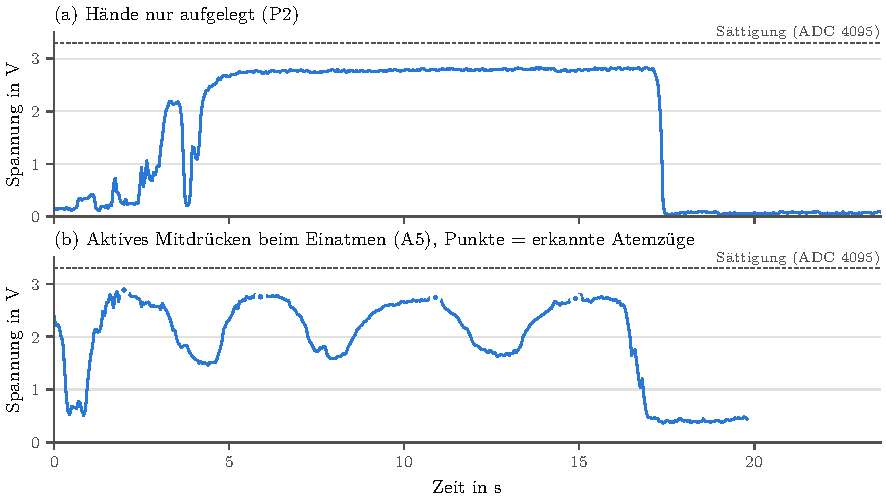
\includegraphics[width=\linewidth]{plots/velostat_aufgelegt_vs_aktiv.pdf}
  \caption{Velostat mit nur aufgelegten Händen (a, P2) und mit aktivem Mitdrücken beim
    Einatmen (b, A5); Punkte markieren die erkannten Atemzüge}
  \label{fig:passiv_aktiv}
\end{figure}

\subsection{Aktive Atemerkennung}
\label{sec:erg_aktiv}

Mit aktivem Mitdrücken zeigten alle sechs Messreihen deutliche, regelmäßige Atemzüge
(Abbildung~\ref{fig:passiv_aktiv}\,b). Der Signalhub lag mit 1410 bis 3360 ADC-Einheiten etwa
drei- bis dreißigmal so hoch wie bei nur aufgelegten Händen. In jedem Auswertefenster wurden vier
bis fünf Atemzüge erkannt; die mittlere Atemperiode lag zwischen 3{,}95 und 6{,}17\,s, was einer
Atemfrequenz von 9{,}7 bis 15{,}2 Atemzügen pro Minute entspricht. In A3 und A4 erreichten 14\,\%
der Werte das obere Ende des Messbereichs, weil zu fest gedrückt wurde; die Atemzüge blieben
trotzdem gut erkennbar. A5 lieferte die saubersten Zyklen ohne Sättigung.

Übertragen auf die Einstufung der Firmware (Abschnitt~\ref{sec:sw_atem}) entsprechen 12{,}1 bis
15{,}2 Atemzüge pro Minute 6 bis 8 Atemzügen in 30\,s und damit der Stufe \enquote{normal}; die
langsamste Messreihe A6 mit 9{,}7 pro Minute läge mit knapp 5 Atemzügen in 30\,s bei
\enquote{entspannt}. Die Ergebnisse sind plausibel, unterliegen aber zwei Einschränkungen: Die
Messungen fanden am Entwicklungsboard und nicht im fertigen Sensoreinsatz statt, und die
Atemzüge wurden offline bestimmt, nicht mit der Erkennung der Firmware.
\todo{Gibt es Tests der Atemerkennung am fertigen Neffy (Erkennungsrate, Einstufung)?}

\subsection{Anwesenheitserkennung}
\label{sec:erg_anwesenheit}

\todoi{Ergebnisse: Ab welcher Entfernung wird eine Person erkannt, wie schnell, Reaktion beim
Vorbeigehen, Fehlauslösungen? Laut Abstimmungsaufnahme der Firmware: direkt davor $+4$ bis
$+6$\,K, in 1\,m etwa $+2$\,K über Raumtemperatur. Messdaten/Logs vorhanden
(\texttt{logs/thermal-*.csv})?}

\section{Evaluation gegen die Anforderungen}
\label{sec:evaluation}

Tabelle~\ref{tab:evaluation} bewertet die Anforderungen aus Tabelle~\ref{tab:anforderungen}.

\begin{table}[htbp]
  \centering
  \caption{Erfüllungsgrad der Anforderungen (\checkmark\ erfüllt, $\circ$ teilweise, -- nicht erfüllt)}
  \label{tab:evaluation}
  \small
  \begin{tabular}{@{}l >{\raggedright\arraybackslash}p{3.6cm}
                    >{\centering\arraybackslash}p{1.3cm}
                    >{\raggedright\arraybackslash}p{6.6cm}@{}}
    \toprule
    Nr. & Anforderung & Status & Begründung \\
    \midrule
    A1 & Anwesenheit erkennen & \todoi{?} & \todoi{Begründung} \\
    A2 & Reaktion auf Anwesenheit & \todoi{?} & \todoi{Begründung} \\
    A3 & Einatemzüge erkennen, Atemfrequenz bestimmen & $\circ$
       & Im Labortest klar erkennbar (9{,}7--15{,}2/min); am fertigen Roboter nicht gemessen
         \todoi{bestätigen} \\
    A4 & Einstufung an den Raspberry Pi & \todoi{?} & \todoi{Begründung} \\
    A5 & Hub mit beiden Händen & \todoi{?} & \todoi{Begründung} \\
    A6 & Gestaltung nach Zielbild & \checkmark
       & Runde, weniger kantige Form mit Taschen umgesetzt \\
    A7 & Hände sicher in Taschen & $\circ$
       & Hände liegen gesichert; Position von Händen und Ellbogen etwas zu hoch \\
    A8 & Zugang zur Elektronik & \checkmark
       & Oberkörper magnetisch, ohne Werkzeug abnehmbar; Unterkörper mit sechs Schrauben \\
    A9 & Druck auf vorhandenen Druckern & \checkmark
       & Alle Teile gedruckt; dafür Teilung in 16 Druckteile nötig \\
    \bottomrule
  \end{tabular}
\end{table}

\section{Schwachstellen}
\label{sec:schwachstellen}

\begin{itemize}
  \item \textbf{Keine passive Atemerkennung:} Das ursprüngliche Ziel, die Atmung allein über die
        aufgelegten Hände zu erkennen, wurde nicht erreicht (Abschnitt~\ref{sec:erg_passiv}). Die
        aktive Erfassung erfordert, dass die Nutzer:innen bewusst mitdrücken.
  \item \textbf{Sättigung bei festem Druck:} Wird zu fest gedrückt, erreicht das Signal das obere
        Ende des Messbereichs (A3, A4). Die Erkennung bleibt möglich, die Signalform geht aber
        verloren.
  \item \textbf{Ergonomie:} Durch die Größe von Neffy~3.0 liegen Hände und Ellbogen etwas zu hoch;
        dieser Punkt wurde im Entwurf zu wenig beachtet. Als einfache Abhilfe dienen kleine Kissen
        links und rechts unter den Ellbogen.
  \item \textbf{Schrittmotoren und Referenzfahrt:} \todoi{Probleme konkret: z.\,B. verlorene
        Schritte, wenn eine Achse beim Start auf dem Endschalter stand; Endlosschleife bei der
        Referenzfahrt des Kopfes (in der Firmware behoben) -- weitere?}
  \item \textbf{Zweckentfremdeter Befehl:} Der Befehl \texttt{DISABLE\_MOTORS} schaltet die Motoren
        nicht ab, sondern dient als Startsignal einer Übung. Der Name passt nicht zur Bedeutung und
        erschwert die Wartung der Schnittstelle.
  \item \textbf{Fertigung:} Es gibt nur eine Gehäuseversion; Toleranzen wurden nicht vorab an
        Testkörpern bestimmt, sodass häufig nachgebohrt werden musste. Die Klebestellen erforderten
        viel Nachbearbeitung.
  \item \textbf{Keine Nutzerstudie:} Anders als zu Neffy~1.0 und 2.0 gibt es zu Neffy~3.0 noch keine
        Evaluation mit Nutzer:innen.
\end{itemize}

\section{Eigene Ideen}
\label{sec:eigene_ideen}

\todoi{Bestätigen bzw.\ ergänzen -- Vorschlag: Übernahme und Umsetzung des gesamten Gehäuses aus
eigener Initiative; modularer Aufbau mit Magneten; Wechsel von passiver zu aktiver Atemerfassung
über die Taschen (zugleich Touch-Eingabe); Sensoreinsatz zum Einstecken; selbstkalibrierende
Klick- und Druckerkennung; lernende Raumtemperatur bei der Anwesenheitserkennung;
LED-Rückmeldung beim Atmen. Wer was (Badre/Younes): ganz am Ende.}

% =====================================================================
%  Kapitel 6 – Fazit (~1 Seite)
% =====================================================================
\chapter{Fazit}
\label{kap:fazit}

\section{Zusammenfassung}
\label{sec:zusammenfassung}

\todoi{Antwort auf die übergeordnete Fragestellung (Abschnitt~\ref{sec:fragestellung}).}

\todoi{Probleme mit den Schrittmotoren, die die Dynamixel-Motoren ersetzt haben
(mehr Kraft benötigt): welche Probleme, Ursachen, Folgen.}

\section{Ausblick}
\label{sec:ausblick}

\todoi{Konkret: Taster statt Velostat, nächste Gehäuseversion, Materialwahl, \dots}

% =====================================================================
%  Kapitel 7 – Einschätzung zum Praktikum (~2–3 Seiten)
%  Ich-/Wir-Form erlaubt.
% =====================================================================
\chapter{Unsere Einschätzung zum Praktikum}
\label{kap:einschaetzung}

\section{Studium und Praktikum}
\todoi{Bezug zu Studieninhalten.}

\section{Praktikumsalltag}
\todoi{Ablauf einer typischen Woche, Laborzeiten; neutral: Verfügbarkeit der Drucker im Labor war eingeschränkt, große Teile (je 15\,h+) mussten eingeplant werden.}

\section{Erwartungen}
\todoi{Erwartungen vorher -- was davon eingetreten ist.}

\section{Erfahrungen}

Fachlich haben wir in diesem Praktikum sehr viel gelernt. Den größten Anteil daran hatte die
Fertigung: Wir haben unsere Kenntnisse in SolidWorks deutlich vertieft, gerade die starken
Rundungen des Gehäuses waren anspruchsvoll zu konstruieren. Beim 3D-Druck großer Teile, beim
Kleben, Schleifen und Lackieren haben wir erfahren, wie viel Zeit und Geduld eine saubere
Oberfläche erfordert, etwa beim Warten zwischen den Lackschichten oder beim Schleifen von Hand.
Dabei haben wir auch gemerkt, wie schnell man an solchen Details perfektionistisch wird.
Überrascht hat uns, wie viel sich durch Kleben lösen lässt; viele der zuvor geplanten
Bohrungen wurden am Ende gar nicht gebraucht.

Hinzu kamen Erfahrungen mit Elektronik: Wir haben viel gelötet, mit dem ESP32 gearbeitet und
gelernt, wie die einzelnen Komponenten im Inneren des Roboters zusammenspielen. Auch Sensoren
wie den Thermalsensor oder Velostat kannten wir vorher nicht. Solche Lösungen können wir uns
gut vorstellen, auch in späteren Projekten wieder einzusetzen.

Innerhalb des Teams Sensorik hat die Zusammenarbeit sehr gut funktioniert. Die Abstimmung mit
den anderen Beteiligten lief ebenfalls gut, wenn sie stattfand, und hat uns jedes Mal
weitergebracht. Viele Entscheidungen mussten wir jedoch selbstständig im Team treffen. Das
zeigte sich am deutlichsten, als wir aus eigener Initiative die Konstruktion des gesamten
Gehäuses übernommen haben. Die meisten Probleme traten während der Entwicklung auf, etwa als
die passive Atemerkennung nicht zuverlässig funktionierte oder die Kupferfolie nicht richtig
leitete. In solchen Situationen mussten wir selbst nach einer Lösung suchen, und das gelang
uns mit der Zeit immer besser.
\todoi{Motivation: Was hat euch angetrieben, was war zäh? (ein bis zwei Sätze)}

\section{Persönliches Fazit}
\todoi{Persönliches Fazit.}


% --- Verzeichnisse ---------------------------------------------------
\listoffigures
\listoftables
\printacronyms
\printbibliography[heading=bibintoc, title=Literaturverzeichnis]

% --- Anhang ----------------------------------------------------------
\appendix
% =====================================================================
%  Anhang
% =====================================================================
\chapter{Code-Auszüge}
\label{anh:code}
\todoi{Atemerkennungs-Modul (.cpp/.h) per \textbackslash lstinputlisting einbinden.}

\chapter{CAD-Zeichnungen}
\label{anh:cad}
\todoi{Technische Zeichnungen des Gehäuses.}

\chapter{Schaltplan}
\label{anh:schaltplan}
\todoi{Schaltplan Neffy Board / Sensoranschluss.}

\chapter{Rohdaten}
\label{anh:rohdaten}
\todoi{Verweis auf Dateien in daten/ bzw.\ Repository.}


% =====================================================================
%  Eigenständigkeitserklärung
% =====================================================================
\chapter*{Eigenständigkeitserklärung}
\addcontentsline{toc}{chapter}{Eigenständigkeitserklärung}

\todoi{Vorgegebenen Wortlaut der BHT bzw.\ des Fachbereichs einsetzen.}

\vspace{3cm}

\noindent
\begin{tabular}{@{}p{6cm} p{6cm}@{}}
  \hrulefill & \hrulefill \\
  Ort, Datum & Eddy Werk \\[2.5cm]
  \hrulefill & \hrulefill \\
  Ort, Datum & Younes Jamil \\
\end{tabular}


\end{document}
